\documentclass[a4paper,12pt]{article}
\usepackage[utf8]{inputenc}
\usepackage[spanish]{babel}
\usepackage{listings}
\usepackage{graphicx}
\usepackage{float}
\usepackage{xcolor}
\definecolor{gris}{RGB}{123, 126, 132}
\definecolor{morado}{RGB}{81, 40, 155}
\definecolor{amarillo}{RGB}{253,151,31}
\definecolor{magenta}{RGB}{249,38,114}

\lstdefinestyle{customJava}{
    frame=tb,
    language=Java,
    backgroundcolor=\color{white},   
    commentstyle=\itshape\color{gris},
    keywordstyle=\bfseries\color{magenta},
    numberstyle=\color{morado},
    stringstyle=\color{amarillo},
    identifierstyle=\color{black},
    basicstyle=\footnotesize,
    breakatwhitespace=false,         
    breaklines=true,                 
    captionpos=b,
    keepspaces=true,                 
    numbers=left,                    
    numbersep=5pt,                  
    showspaces=false,                
    showstringspaces=false,
    showtabs=false,                  
    tabsize=2,
}

\renewcommand{\lstlistingname}{Código}

%opening
\title{Tarea No. 12. Ciclo de vida de Hibernate}
\author{Barrera Pérez Carlos Tonatihu \\ Profesor: José Asunción Enríquez 
Zárate \\ Web Application Development \\ Grupo: 3CM9 }

\begin{document}

\maketitle
\newpage
\tableofcontents
\newpage

\section{Introducción}
Hibernate es todo un mundo en cuanto al desarrollo de aplicaciones que 
interactúen con una fuente de datos mediante un ORM por lo que entender el 
ciclo de vida de Hibernate es clave en su uso, es por esto que en esta tarea se 
explicara en que consiste este tema.
\section{Desarrollo}
El ciclo de vida de Hibernate muestra el como los objetos persistentes son 
manejados. Hibernate guarda, actualiza y borra registros en las tablas de la 
base de datos con respecto al valor del objeto ya que su clase persistente está 
asociada con la tabla de la base de datos. Como se puede observar en 
la figura \ref{fig:diagrama} Hibernate presenta los siguientes estados.


\begin{figure}[H]
    \begin{center}
    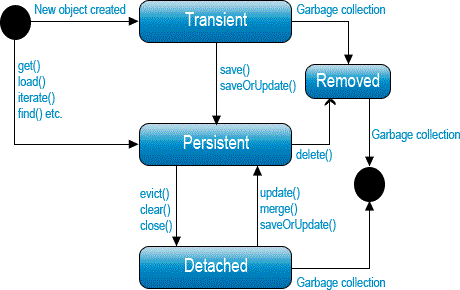
\includegraphics[width=\textwidth]{diagrama.png}
    % estructura.png: 800x436 px, 96dpi, 21.16x11.53 cm, bb=0 0 600 327
    \caption{Ciclo de vida de Hibernate}
    \label{fig:diagrama}
    \end{center}
\end{figure}

\subsection{Transient}
Cuando creamos un objeto de nuestra clase POJO podemos decir que se encuentra 
en el estado trasient. En este estado no se encuentra relacionado con ninguna 
tabla de la base de datos, por lo que cualquier modificación no afecta a la 
base de datos. Si ya no es referenciado por algún objeto pasa al garbage 
collection. Por ejemplo.

\begin{lstlisting}[language=Java,style=customJava,basicstyle=\fontfamily{cmss}
\small]
Empleado empleado = new Empleado // Objeto es estado transient
\end{lstlisting}

\subsection{Persistent}
Cuando se guarda un objeto transient entra en estado persistent. En este estado 
tiene una fila de alguna tabla de base de datos asociada con una llave 
primaria. es inicializado por el manejador de persistencia cuando se llama el 
método save(). Si ya existe en la base de datos se puede recuperar. Y todos los 
cambios hechos en este estado son guardados automáticamente.

Se puede obtener un objeto persistente al utilizar alguno de estos metodos en 
una sesión de Hibernate.
\begin{itemize}
 \item save()
 \item update()
 \item saveOrUpdate()
 \item lock()
 \item merge()
\end{itemize}

Un ejemplo de esto es el siguiente código.
\begin{lstlisting}[language=Java,style=customJava,basicstyle=\fontfamily{cmss}
\small]

Session session = Session.getCurrentSession();

Empleado empleado = new Empleado(); // Estado transient
session.saveOrUpdate(empleado); // Estado persistent

empleado.setNombre("Carlos"); // Modificacion es guardada

session.getTransaction().commit(); // Commit a la transaccion

\end{lstlisting}

\subsection{Detached}
En este estado el objeto persistente continua existiendo después del cierre de 
la sesión activa. Se puede decir que un objeto detached se mantiene despues de 
que termina una transacción por lo que continua representando una fila valida 
de la base de datos.

Los cambios hechos en este tipo de objetos no son guardados en la base de 
datos, para entrar en este estado se utiliza el método evict() o en la sesión 
se utiliza se utiliza el método clear() o close(). Para volver a hacer un 
objeto persistente se pueden llamar a los siguientes métodos.

\begin{itemize}
 \item update()
 \item merge()
 \item saveOrUpdate()
 \item lock()
\end{itemize}

\subsection{Removed}
Cuando el objeto persistente es borrado de la base de datos pasa el estado de 
removido, para hacer esto se utiliza el método delete(). Un ejemplo de esto es 
lo siguiente.

\begin{lstlisting}[language=Java,style=customJava,basicstyle=\fontfamily{cmss}
\small]
Session sesion = Session.getCurrentSession();
Empleado empleado = sesion.get(Empleado.class, 2);
sesion.delete(empleado);
empleado.setName("Juan"); // Esto ya no tiene efecto
sesion.getTransaction.commit();
\end{lstlisting}

\section{Conclusiones}
Hibernate tiene una gran cantidad de conceptos clave para poder utilizarlo 
correctamente, este es uno de los más fundamentales debido a que al momento de 
estar trabajando con entidades se pueden presentar bastantes problemas y si no 
entendemos el ciclo de vida pude volver la resolución de estos problemas algo 
más complicado de lo que seria en un principio.

\end{document}
